%----------------------------------------------------------------------------
\chapter{Hardware and software environment}\label{chap:Environment}
%----------------------------------------------------------------------------
%Glossary entries
\newglossaryentry{utc}{name=UTC, description={Coordinated Universal Time}}
\newglossaryentry{pqr}{name=PQR, description={Coordinated Universal Time}}
%----------------------------------------------------------------------------
The primary task of the SOLSUN Traffic Sensor is counting, that is performed by the core software.
However, since the system is nested into its surroundings, it requires other supplementary software that facilitates the operation in the production environment on the target hardware, connects the Sensor to the user, and provides diagnostic tools for testing and evaluation.

The aim of this section is to offer an insight into the operation and structure of the hardware and software environment of the Sensor.
Although the supplementary elements are integral parts of the system, their characteristics will be merely sketched without going into detail, because they are out of the main scope of this thesis work.
For further detail, see the work of Tam{\'a}s T{\'o}th \cite{Toth2016}.
%---------------------------------------------------------------------------
\section{Hardware environment}
%----------------------------------------------------------------------------
\subsection{The target board}
Since the hardware will be installed inside a street-lighting lamp box, it must be able to function using a passive cooling system.
The target hardware, chosen to suit this requirement, is an UDOO Quad minicomputer using a small and effective Ubuntu Linux-based UDOObuntu 2 operating system.
The board has an i.MX6 ARM\reg Cortex\reg-A9 Quad, \SI{1}{GHz}, multi-core CPU \cite{UDOO, UDOO2}.
A CSI camera interface and a USB 2.0 port is available on the hardware, for connecting the camera.

\subsection{Network architecture and communication}
The Sensor instances deployed into the lamp boxes communicate with each other and the central server via a radio frequency (RF) channel, that uses an open, ISM (Industrial Scientific Medical) band.
Although RF communication has limited bandwidth, since only a rather small amount of information (only the result of the counting) is transmitted, it is sufficient for this purpose.
Data transmission is mediated by the EnTalk\textsuperscript{TM} communication protocol\cite{EnTalk}.
The sending and receiving of the information is organized as a multi-hop mesh system, wherein each communication node is connected solely to its direct neighbours, namely the two closest lamp posts (as seen in figure \ref{fig:network}).
This way, the short range of RF communication cannot impede the data transfer.

\begin{figure}[!h]
	\centering
	\includegraphics[width=0.5\textwidth]{network.png}
	\caption[The structure of the multi-hop mesh network]{The structure of the multi-hop mesh network. For a short-ranged communication, each node transfers the information to its closest neighbours. \label{fig:network}}
\end{figure}

The server communicates through an API (Application Programming Interface), that implements the REST (Representational State Transfer) principles. 
In both directions JSON (JavaScript Object Notation) syntax files are transmitted.
Each node is identified by the server with an EnTalk\textsuperscript{TM} ID.
%----------------------------------------------------------------------------
\section{Supplementary software elements}\label{sec:SupplementarySoftware}
%---------------------------------------------------------------------------
The auxiliary software elements' main responsibility is connecting the core to its surroundings.
They provide access to the sensor by transferring the input data (e.g. settings files, software upgrades), from the user to the core software, and returning information (such as the result of counting and diagnostics data) to the backend server, via the EnTalk\textsuperscript{TM} connection.
An overview of the transmission procedure is seen in figure \ref{fig:environment}.

\begin{figure}[!h]
	\centering
	%\includesvg[width=0.75\textwidth]{environment}
	\includegraphics[width=0.75\textwidth]{environment.png}
	\caption[The environment of the core software]{The structure of the core software's environment. The core software runs on an UDOO Board built inside a lamp post, and connects to a camera that is continuously monitoring the road. Data is transmitted through a multi-hop mesh network, the EnTalk\textsuperscript{TM} Network. From the Traffic Sensor to the server, regular reports are sent, and diagnostics data is transmitted as an answer to the control commands. From the server to the core software control commands, software updates and settings files are sent to the sensor. \label{fig:environment}}
\end{figure}

The supporting software has various other features.
The configuration tools facilitate the operation under heterogeneous circumstances by providing the ability to set individual settings for each environment.
Diagnostics tools evaluate the operation and visualize the data stored in the system in various representations, and are also responsible for the exporting of the result of counting, classification and quantified diagnostics in text files.
%----------------------------------------------------------------------------
\subsection{Communication}\label{sec:communication}
%----------------------------------------------------------------------------
\subsubsection{Reporting}\label{sec:reporting}
At the production environment the Sensor operates continuously, and the result of the detection is regularly sent through the EnTalk\textsuperscript{TM} connection as JSON syntax report file. 
This reporting procedure is periodical, and the time interval of each period can be set as a configuration parameter.
The report file contains the number of counted vehicles in each category along with their average speed and following distance.
An example is shown in code-listing \ref{lst:report_file}.

\begin{lstlisting}[frame=single,float=!ht,caption={Part of a report file. The result of the counting is sent as a JSON syntax file, including the number of vehicles detected in each category.},label=lst:report_file]
{
	"entalkid" : "BMETS001",
	"pid" : 8,
	"period" : 300,
	"sampleutc" : 1453740815,
	"samples":
			{
				"cars":
				{
					"count" : 10,
					"avg_speed" : 24.8,
					"avg_distance" : 5.8
				},
				"trucks":
				{
					"count" : 5,
					"avg_speed" : 23.9,
					"avg_distance" : 7.1
				},
				...
				"total_objects" : 37
			}
}
\end{lstlisting}

The reporting is part of the regular operation of the Sensor, that is core software's responsibility.
Other irregular control and management functions are handled by the Project Configurator application, and are detailed in the following section.

\subsubsection{Remote management}
Since the Sensors are installed in street-lighting lamp boxes high above the road, where accessed with difficulty, and will be deployed en masse, control functions and software upgrades must be managed remotely.

To achieve this, each instance of the sensor can be accessed through a graphical user interface (GUI), the Project Configurator.
The Project Configurator itself is a separate, autonomous application of the Traffic Sensor system.
The GUI is show in figure \ref{fig:project_configurator}.
Although it is in charge of a handful of tasks, including the manual configuration of the calibration features (detailed in section \ref{chap:calibration}), its main purpose is to enable the remote control of the Sensors by managing the EnTalk\textsuperscript{TM} communication.

The management functions include the uploading of calibration files and new software versions (updates) to the sensor, and the downloading of log files and diagnostics data (such as images and calibration videos).
The UI is capable of sending control commands as well.
%----------------------------------------------------------------------------
\subsection{Configuration}\label{subs:ProjectConfigurator}
%----------------------------------------------------------------------------
Since the position of the camera and the surrounding environment of the Traffic Sensor are undetermined and varying, the system's properties has to be adjustable to meet the particular requirements.
To be able to calibrate the Traffic Sensor's several parameters in a group, a two-level configuration method was implemented.
The system's settings are listed in two separate files, the settings file and the project file.
These are standard INI format files, each of them specifying parameters and their values as key--value pairs, grouped into sections as seen in code-listing \ref{lst:config_file}.

\begin{lstlisting}[frame=single,float=!ht,caption={Part of a configuration file. Features are organized into sections, and presented as key--value pairs.},label=lst:config_file]
[mog2]
backgroundRatio = 0.95
complexityReductionThreshold = 0.1
shadowDetection = true
history = 300
nMixtures = 4
shadowThreshold = 0.5
shadowValue = 0
varInit = 15.0
varMax = 75.0
varMin = 4.0
varThreshold = 35.0
varThresholdGen = 9.0
maxWhitenessPercentage = 15.0
blacknessHoldCountAfterOverreaction = 40

[VideoFrameTransform]
enable = true
targetWidth = 320
targetHeight = 240
perspectiveCompensation = true
tripwireRotation = true
processLanesOnly = false
pixelRowPerLane = 5
laneClearance = 5

[CalibrationCorrection]
slopeThreshold = 0.15

[Output]
RecordDemoVideo = false
Evaluation = true
...
\end{lstlisting}

On the first level, the settings file contains basic configuration values, as default parameters for the operation.
Each of these properties can be overridden by the specifications listen is the project file if needed, for an environment-specific configuration.

Most of the listed properties are algorithm parameters, e.g. threshold values for image processing methods.
Other parameters affect the operation by specifying the run mode (discussed further in section \ref{sec:run_modes}), changing the report frequency and the maximal number of stored timeline columns, or deactivating processing steps.
Some properties are strictly environment-specific, like the position of the Tripwire in the frame, and the calibration rectangle.
The visualization and saving of miscellaneous media -- e.g. timeline images, videos and diagnostics files -- can be switched on and off as well.

\subsection{Calibration}\label{chap:calibration}
%----------------------------------------------------------------------------
Some environment-specific parameters can be manually configured using the aforementioned Project Configurator GUI.
The position of the Tripwire, the calibration rectangle, and optionally, the centre of road-lanes can be set and adjusted.
To specify these features, the user simply draws on a proper frame, chosen from a short video sequence, that is recorded form the camera, or read from the video file by the Configurator itself.
Other numeric parameters, like the beginning and ending frame of the video, or the length of the sides of the calibration rectangle can be pre-set as well.
The GUI is able to write the specified values into the appropriate configuration file, and send the file to the Sensor. 

\begin{figure}[!h]
	\centering
	\includegraphics[width=0.5\textwidth]{projectConfigurator.png}
	\caption[The GUI of the Project Configurator]{The user interface of the Project Configurator. Using the GUI several parameters can be set, including the Tripwire (with lilac), the calibration rectangle (with yellow), and other numeric values in text input fields. The Tripwire's beginning and ending point determine the order, in which its pixels are processed. Since the Project Configurator can read, write and upload configuration files to the Sensor, the above functions can be managed jointly through the GUI. \label{fig:project_configurator}}
\end{figure}
%----------------------------------------------------------------------------
\subsection{System diagnostics}\label{sec:system_diagnostics}
%----------------------------------------------------------------------------
The system diagnostics features are responsible for evaluating the precision of the operation and converting information stored, into a simply interpretable form.
%----------------------------------------------------------------------------
\subsubsection{Evaluation}\label{chap:evaluation}
To quantify the accuracy of the operation, the system was tested on a series of test videos.
The videos were recorded in various weather, light and traffic conditions to ensure the system's robustness.

To be able to evaluate the performance of the counting, the correct detection and classification values were gathered into a reference data set, called the ground truth, and were compared to the results of the counting.
The data set is created manually, based on the Original Timeline Image of the corresponding video stream of each test video.

\begin{figure}[!h]
	\centering
	\begin{subfigure}[!h]{0.87\textwidth}
		\includegraphics[width=\textwidth]{original_GT.png}
		\caption{Original timeline, each vehicle is dotted with a colour, depending on its type.\label{fig:GT_original}}
	\end{subfigure}
	\hfill
	\begin{subfigure}[!h]{0.87\textwidth}
		\includegraphics[width=\textwidth]{GT_GT.png}
		\caption{Ground truth image.\label{fig:GT_GT}}
	\end{subfigure}
	\hfill
	\begin{subfigure}[!h]{0.87\textwidth}
		\includegraphics[width=\textwidth]{MOG2_GT.png}
		\caption{GT points matched with the detected vehicles. \label{fig:GT_MOG}}
	\end{subfigure}
	\hfill
	\begin{subfigure}[!h]{0.87\textwidth}
		\includegraphics[width=\textwidth]{result_GT.png}
		\caption{The result of the evaluation. True positive cases are marked with neutral colours, false positive cases are crossed out with red, blue dots indicate false negative errors.\label{fig:GT_result}}
	\end{subfigure}
	\caption[The creation of the reference data set, the ground truth]{The creation and evaluation process of the reference data set, the ground truth.\label{fig:GT}}
\end{figure}

A ground truth file can be considered itself as an image, with points that match the vehicles of the Original Timeline.
Every point is marked with a coloured dot, with the colour indicating the type of the vehicle.
At the end of the process, the detection results are compared to the GT's  points, and precision is evaluated based on the error rates of the comparison.

\begin{figure}[!h]
	\centering
	%\includesvg[width=0.35\textwidth]{error_cases}
	\includegraphics[width=0.35\textwidth]{error_cases.png}
	\caption[Possible error cases]{Possible error cases, and their markings on the Evaluation Result Timeline. Misclassification errors are not indicated, however can be visualized separately on the Misclassification Error Timeline.\label{fig:error_cases}}
\end{figure}

For evaluation the following typical binary classification cases were used (as shown in figure \ref{fig:error_cases}):
\begin{enumerate}
\item \textbf{TP -- true positive:} correctly detected vehicles, where a vehicle in the MOG2 Timeline matches a point in the GT image.
\item \textbf{FP -- false positive:} a vehicle was detected, but has no matching point in the GT image.
\item \textbf{FN -- false negative:} no vehicle was detected, but a point is present in the GT. 
\item \textbf{TN -- true negative:} true negative cases are undefined.
\item  \textbf{CC -- correct classification:} the point in the GT and the matching vehicle are the same types.
\end{enumerate}

The above abbreviations have two distinct meanings. 
First, they refer to instances of the described cases, and in the second place, in equations, they mark the number of cases found whilst evaluating a specific test video.

To quantify the performance of the system, the following measures -- also known in binary classification theory -- were used:
\\[5pt]
\noindent Recall:
\begin{displaymath}
\text{R} = \frac{\text{TP}}{\text{TP}+\text{FN}} = \frac{\text{TP}}{\text{NGP}}
\end{displaymath}
\\[5pt]
\noindent Accuracy:
\begin{displaymath}
\text{A} = \frac{\text{TP}+\text{TN}}{\text{NAC}} = \frac{\text{TP}}{\text{NAC}} = \frac{\text{TP}}{\text{TP}+\text{FP}+\text{FN}}
\end{displaymath}
\\[5pt]
\noindent False positive rate:
\begin{displaymath}
\text{FPR} = \frac{\text{FP}}{\text{NAC}}
\end{displaymath}
\\[5pt]
\noindent False negative rate:
\begin{displaymath}
\text{FNR} = \frac{\text{FN}}{\text{NAC}}
\end{displaymath}
\\[5pt]
\noindent Type recall:
\begin{displaymath}
\text{TR} = \frac{\text{CC}}{\text{TP}},
\end{displaymath}

with $\text{NAC}$ being the number of all cases, and $\text{NGP}$ is the number of GT points.
For each test video, the aforementioned measures were calculated.
The experimental results are presented in chapter \ref{chap:Tests} in detail.
%----------------------------------------------------------------------------
\subsubsection{Data representation}\label{sec:data_representation}
%----------------------------------------------------------------------------
The Traffic Sensor software supports several features for converting the raw information stored in the system into a form for human interpretation.
The exportation of visual information is assigned to the Output Builders classes.

The main diagnostic feature is the exportation of the data in the form of the following timeline images.
\begin{enumerate}
	\item \textbf{Untransformed Timelines -- Original, MOG2 Timeline: } Exported directly from the raw data stored.
	\item \textbf{Transformed Timelines -- Speed, Size, Following Distance Timeline: } The raw image data is rescaled, normalized and optionally assigned to three channels before saving. The lightness of the pixels indicate a higher original numeric value. Speed values are marked with either red or blue depending on the direction of the movement. 
	\item \textbf{Blob Timeline: } The found vehicles, stored in the vehicle storage object, drawn on a Timeline Image. Different from the MOG2 Timeline, because after the blobs of the MOG2 Timeline Image are counted, the found objects are post-corrected. The post corrections include size-filtering, the fusion of separated blobs, and the reconnection of the split objects.
	\item \textbf{Result Timeline: } Similar to the Blob Timeline, the Result Timeline contains vehicle occurrences, each of them drawn with a separate colour. Other features, such as size, average speed and vehicle type can be displayed as well.
	\item \textbf{Evaluation Timeline: } The Evaluation Timeline shows the result of the evaluation, each classification case (described in section \ref{chap:evaluation}) marked perceptively.
	\item \textbf{Error Timeline Images: } For each error type (false positive, false negative, misclassification error) a Timeline Image can be exported, showing only the respective error cases.
\end{enumerate} 
The Timelines are either saved in their raw state (e.g MOG2 Timeline), transformed into a more visually understandable form (e.g. Speed Timeline), or the contents of container objects are drawn on blank Timeline Images (like Blob Timeline, Error Timelines).
Some examples of the visualizations of Timelines are found in appendix \ref{app:TIs}.

Depending on the operation mode of the Traffic Sensor (discussed in section \ref{chap:operation_modes}), either complete Timeline Images can be saved at the end of the full process, or parts of them can be exported periodically, each time the size of the stored data overruns a pre-defined limit.

The system is able to build and save video files for demonstration purposes as well, namely a raw video sequence (with the intention of manual calibration in the Project Configurator, or later testing), and a demo video file with user-defined frame structure for demonstration.
The demo video frames can be made up by any Frame-strip or Timeline Image, along with the visualization of counting statistics.
An example of a demo video frame is shown in figure \ref{fig:demo_video}.

The result of the calibration correction can be displayed as well, in the form of two images, containing the measured average vehicle lengths along the Tripwire, or the original calibration rectangle with the revised one. 
An example of these images are shown in figure \ref{fig:cal_corr_example}, and the calibration correction process is further detailed in section \ref{chap:cal_corr}.

\begin{figure}[!h]
	\centering
	\includegraphics[width=0.5\textwidth]{frame_demo_vide.png}
	\caption[Example frame from the demo video]{An example frame from the demo video. The desired structure of the demo video frame is defined in the configuration files.  \label{fig:demo_video}}
\end{figure}

Along with the report files containing the result of the counting in a JSON format, it is possible to export other characteristic information as text files.
The diagnostic files are as follows:
\begin{enumerate}
	\item \textbf{Log file: } Contains the timing values of the operation. Used for speed-testing purposes. Evaluated during the run on the target hardware.
	\item \textbf{Evaluation result file: } Displays the numeric results of evaluation. The number of each cases and the value of the calculated measures (defined in section \ref{chap:evaluation}) are listed in an HTML (Hypertext Markup Language) format file.
	\item \textbf{Corrected calibration rectangle: } This file contains the plain list of the edges of the corrected calibration rectangle, can be copied later to redefine the original edges.
\end{enumerate}

\begin{figure}[!h]
	\centering
	\begin{subfigure}[b]{0.4\textwidth}
		\includegraphics[width=\textwidth]{calibrationCorrection_not_OK_GoldB1_Sun.png}
		\caption[Visualization of sverage vehicle lengths along the Tripwire]{Average vehicle length values along the Tripwire. All length data are in meter.}
	\end{subfigure}
	\quad
	\begin{subfigure}[b]{0.4\textwidth}
		\includegraphics[width=\textwidth]{calibratedRectangle.png}
		\caption{The corrected calibration rectangle (with blue) drawn over the original one (with yellow).}
	\end{subfigure}
	\caption{The result and diagnostics data of the calibration correction exported as images.\label{fig:cal_corr_example}}
\end{figure}

The videos, calibration correction frames, and result files can be exported by the Sensor at the end of the operation (in single-run mode), and timeline images and log files during (in continuous mode).
The exported files can be remotely downloaded using the Project Configurator.

%----------------------------------------------------------------------------
\subsubsection{Continuous integration tests}\label{sec:continuous_integration}
%----------------------------------------------------------------------------
To test the proper operation of the system at all times, and to ensure discovering potential errors at the earliest possible, a functional test script runs automatically each nigh.
The script compiles and runs the latest Traffic Sensor version accessible in the version control system.
The results of the operation are then shortly shared via an on-line interface with the developers.
%----------------------------------------------------------------------------
\section{Operation modes of the Traffic Sensor}\label{chap:operation_modes}
%----------------------------------------------------------------------------
Depending on the particular situation and the user's aim, the Traffic Sensor is able to function in two different operation modes (shown in figure \ref{fig:run_types}).
%----------------------------------------------------------------------------
\subsubsection{Single-run or test mode}\label{sec:run_modes}
First, for testing, development and evaluation purposes the single-run mode is used.
The input video is a file or a stream from a camera, both with a specified number of frames to be processed.
Since in the single-run mode the process has an exact end, thus the length of the procedure is known, it is possible to create GT files in advance, and at the close of the operation, be evaluated.
Post-corrections, like calibration correction are possible as well.
At the end of the procedure, other files, such as entire Timeline Images and video files, including the recorded video stream, or a demo video are created and exported using the data collected throughout the process.
Although most output files are generated at the end of the operation, reporting is iterative.
The Sensor sends a report every time after a fixed time interval -- specified in the configuration files-- has elapsed.

\begin{figure}[htb]
	\centering
	%\includesvg[width=\textwidth]{process_run_types}
	\includegraphics[width=\textwidth]{process_run_types.png}
	\caption[Operation modes of the Traffic Sensor]{Operation modes of the Traffic Sensor. The single-run mode is for testing and development (above), when a video file or a stream with a pre-set count of frames is processed. The single-run mode has a definite ending, when post-process evaluations and tests are carried out, and entire Timeline Images are saved. In the production environment, the Sensor functions in a continuous mode. Since the amount of memory is finite, and the end of the process is not predictable, in continuous mode, all events happen periodically. The only exception is reporting, that happens regularly after fixed intervals in both run modes. \label{fig:run_types}}
\end{figure}
%----------------------------------------------------------------------------
\subsubsection{Continuous run}
%----------------------------------------------------------------------------
For constant operation it the production environment, the continuous run mode is used.
During continuous run, all milestone events, such as reporting and TI saving, are periodic. 
Detection takes place during the course of each period. 
Meanwhile, columns of the required output Timeline Images are collected for saving.
Considering that the memory of the target hardware is limited, Timeline Images are built and saved in parts with pre-defined lengths.

At the end of the iteration, the collected Timeline Image columns are exported in a png image format, and results of detection and classification are sent as a report file.
In this mode evaluation and correction features are not accessible.